% Frames

% Attack => Et attack paa det eksempel Dennis gennemgaar  (scenariet)

% Countermeasures => Vis hvordan et countermeasure kunne vaere implementeret paa det eksempel

\begin{frame}[fragile]{Introduction}
\begin{center}
	\begin{itemize}
	\item Smart cards are increasingly being integrated in every day life (credit cards, Rejsekort, etc.)
	\item Estonia uses smart cards as national cards \footnote{https://e-estonia.com/component/electronic-id-card/}
		\begin{itemize}
		\item[-] Travel within EU borders
		\item[-] Health insurance card
		\item[-] e-Prescriptions
		\item[-] Other countries are interested in their solution
		\end{itemize}
	\end{itemize}
\end{center}
\end{frame}

\begin{frame}[fragile]{\large How can bit flips be introduced and why are they a problem?}
Bit flips can present security issues, such as validation bypassing and control of other applets on a smart card\\~\\
Different sources:\\~\\
	\begin{itemize}
	\item Cosmic rays
	\item Packaging
	\item Lasers
	\item Heat
    \item Electrical equipment\\~\\
	\end{itemize}
	
The sources have different levels of precision
\end{frame}
\begin{frame}[fragile]{Field of Bit \& Instruction Differentiation}
\begin{itemize}
\item What if FoB was not implemented in the JCVM?
\end{itemize}
\begin{table}
\centering
\begin{tabular}{|c|c|c|c|c|c|}
\hline PC & 4 & 5 & 6   \\ 
\hline ifeq & X & R & R \\ 
\hline goto & X & R & R \\ 
\hline newInst & X & R & X \\ 
\hline 
\end{tabular} 
\end{table}
\end{frame}

\begin{frame}[fragile]{Field of Bit \& Instruction Differentiation}
\begin{minipage}{.45\textwidth}
\begin{lstlisting}[frame=single]
...
 1: invokespecial #6
 4: ifeq 15
 7: new           #3
10: dup
11: invokespecial #7
14: athrow
15: aload_0
16: invokespecial #8
...
\end{lstlisting}
\end{minipage}%
\hspace{20px}
\begin{minipage}{0.45\textwidth}
\begin{lstlisting}[frame=single]
...
 1: invokespecial #6
 4: goto 15
 7: new           #3
10: dup
11: invokespecial #7
14: athrow
15: aload_0
16: invokespecial #8
...
\end{lstlisting}
\end{minipage}
\begin{center}
$ifeq = 0x60,\:goto = 0x70$
\end{center}
\end{frame}

\begin{frame}[fragile]{Field of Bit \& Instruction Differentiation}
\begin{itemize}
\item What if FoB was not implemented in the JCVM?
\item Mapping of instructions to opcodes could be changed to improve security
\end{itemize}
\begin{table}
\centering
\begin{tabular}{|c|c|c|c|c|c|}
\hline PC & 4 & 5 & 6   \\ 
\hline ifeq & X & R & R \\ 
\hline goto & X & R & R \\ 
\hline newInst & X & R & X \\ 
\hline 
\end{tabular} 
\end{table}
\end{frame}

\begin{frame}[fragile]{Our Solution}
\begin{center}
\begin{figure}
\def\svgwidth{\columnwidth}
%% Creator: Inkscape inkscape 0.48.4, www.inkscape.org
%% PDF/EPS/PS + LaTeX output extension by Johan Engelen, 2010
%% Accompanies image file 'workflow_new_blank.pdf' (pdf, eps, ps)
%%
%% To include the image in your LaTeX document, write
%%   \input{<filename>.pdf_tex}
%%  instead of
%%   \includegraphics{<filename>.pdf}
%% To scale the image, write
%%   \def\svgwidth{<desired width>}
%%   \input{<filename>.pdf_tex}
%%  instead of
%%   \includegraphics[width=<desired width>]{<filename>.pdf}
%%
%% Images with a different path to the parent latex file can
%% be accessed with the `import' package (which may need to be
%% installed) using
%%   \usepackage{import}
%% in the preamble, and then including the image with
%%   \import{<path to file>}{<filename>.pdf_tex}
%% Alternatively, one can specify
%%   \graphicspath{{<path to file>/}}
%% 
%% For more information, please see info/svg-inkscape on CTAN:
%%   http://tug.ctan.org/tex-archive/info/svg-inkscape
%%
\begingroup%
  \makeatletter%
  \providecommand\color[2][]{%
    \errmessage{(Inkscape) Color is used for the text in Inkscape, but the package 'color.sty' is not loaded}%
    \renewcommand\color[2][]{}%
  }%
  \providecommand\transparent[1]{%
    \errmessage{(Inkscape) Transparency is used (non-zero) for the text in Inkscape, but the package 'transparent.sty' is not loaded}%
    \renewcommand\transparent[1]{}%
  }%
  \providecommand\rotatebox[2]{#2}%
  \ifx\svgwidth\undefined%
    \setlength{\unitlength}{361.0997458bp}%
    \ifx\svgscale\undefined%
      \relax%
    \else%
      \setlength{\unitlength}{\unitlength * \real{\svgscale}}%
    \fi%
  \else%
    \setlength{\unitlength}{\svgwidth}%
  \fi%
  \global\let\svgwidth\undefined%
  \global\let\svgscale\undefined%
  \makeatother%
  \begin{picture}(1,0.18633991)%
    \put(0,0){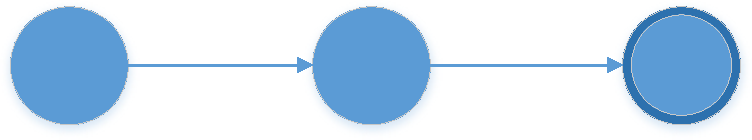
\includegraphics[width=\unitlength]{figures/workflow_new_blank.pdf}}%
    \put(0.09240599,0.11){\color[rgb]{1,1,1}\hspace{-5px}\parbox[t]{0pt}{\tiny{1:} \\ \makebox(0,0)[b]{\hspace{10px}\tiny{Java bytecode}}}}%
    \put(0.23582069,0.11082579){\color[rgb]{.4,.4,1}\makebox(0,0)[lb]{\footnotesize{\textit{conversion}}}}%
    \put(0.57628484,0.11082579){\color[rgb]{.4,.4,1}\makebox(0,0)[lb]{\textit{\footnotesize{property verification}}}}%
    \put(0.49614524,0.11){\color[rgb]{1,1,1}\hspace{-5px}\parbox[t]{0pt}{\tiny{2:} \\ \makebox(0,0)[b]{\hspace{10px}\tiny{UPPAAL model}}}}%
    \put(0.90772511,0.11){\color[rgb]{1,1,1}\hspace{-5px}\parbox[t]{0pt}{\tiny{3:} \\ \makebox(0,0)[b]{\hspace{10px}\tiny{Assessment}}}}%
  \end{picture}%
\endgroup%

\caption{The workflow of the solution, from Java bytecode to UPPAAL SMC model and assessment of the modelled program.}
\label{fig:workflow_new}
\end{figure}
\end{center}
\end{frame}

%\begin{frame}[fragile]{Modelling Multiple Bit Flips in UPPAAL}
%\begin{itemize}
%\item Limitations of current fault model
%\subitem Semantics for describing failed reads / writes
%\item Multiple bit flips	
%\end{itemize}
%\end{frame}

\begin{frame}[fragile]{Extended Solution}


\begin{figure}
\centering
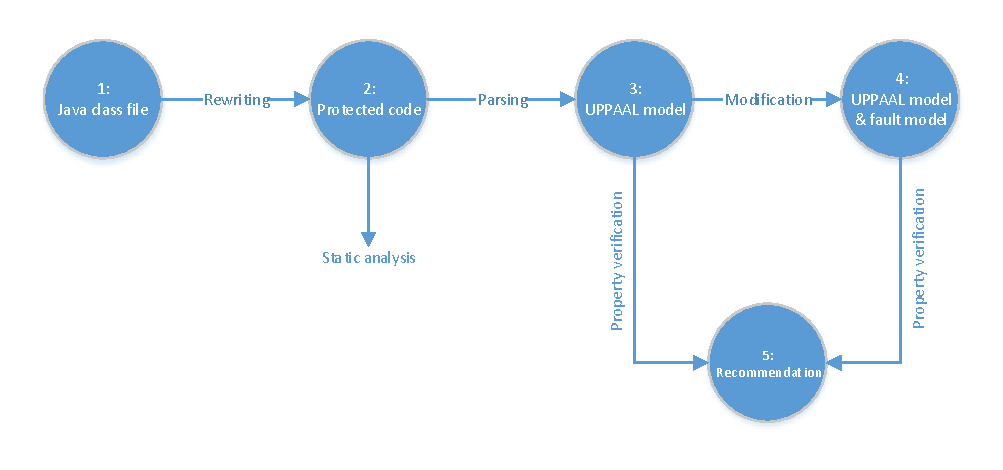
\includegraphics[scale=0.65]{figures/workflow.pdf}
\caption{\footnotesize The extended solution, consisting of automatic rewriting, UPPAAL SMC model conversion, fault injection and countermeasure recommendation.}
\label{test}
\end{figure}
\end{frame}